\section{Analysis applications and services} \label{sec:apps}

TOKIO's connector and tool interfaces are simply mechanisms to access I/O telemetry from throughout an HPC center.
As illustrated in Figure \ref{fig:portability-flow}, a higher-level analysis application is required to actually connect pytokio's interfaces to meaningful insight to an end-user.
To demonstrate how such an analysis application may be built on top of pytokio, pytokio includes a number of example applications and services that broadly fall into three categories: command-line interfaces into pytokio, statistical analysis tools, and data and analysis services.

\subsection{Command-line interfaces to pytokio} \label{sec:apps/cli}

Many connectors and tools present methods and functions that are valuable for users as-is.
For example, being able to retrieve application-level I/O performance telemetry with a single job id (as was presented in Section \ref{sec:architecture/tools}) is an intrinsically useful operation.
To expose such useful functions directly to users without requiring that they write python, pytokio includes a set of command-line tools that simply convert command-line options into input arguments, pass these arguments to a single pytokio function, and then return the resulting output as ASCII to stdout.

Perhaps the most immediately valuable tools of this category are the command-line interfaces for each connector's serialization method, which allow specific component-level data to be quickly serialized into a generic and portable format.
For example, the LMT connector allows the contents of the LMT MySQL database to be serialized to a local SQLite file.
By serializing this data during a time period of interest, LMT data can be analyzed long after the 24-hour window in which LMT database retains data.
Furthermore, because the data is serialized to a standard and portable format, the SQLite database file itself can be shared and analyzed on remote systems for purposes of collaboration or reproducibility.

\subsection{Statistical analysis tools} \label{sec:apps/analysis}

\begin{figure}[t]
    \centering
    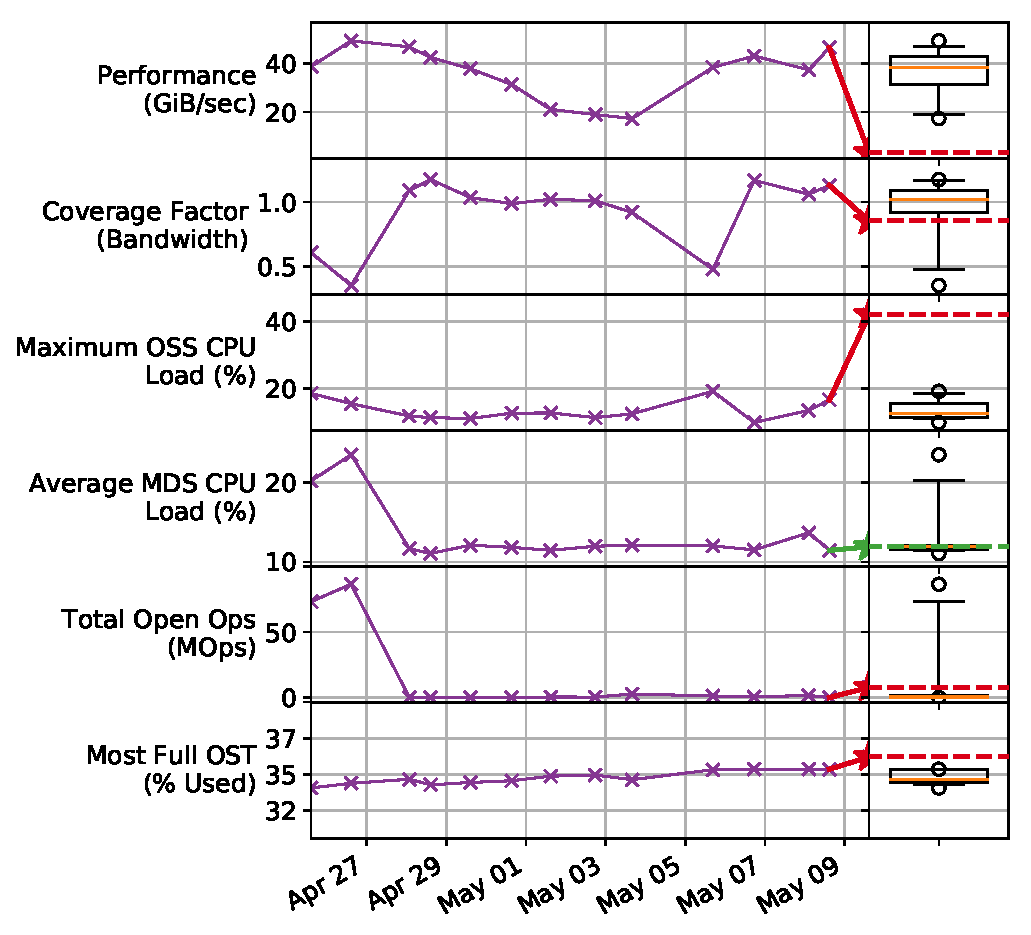
\includegraphics[width=1.0\columnwidth]{theta-umami}
    \vspace{-.3in}
    \caption{UMAMI diagram of a simulated science campaign of BD-CATS~\cite{patwary2015bd} simulations performed on ALCF's Theta system.  
    "Coverage Factor (Bandwidth)" is the fraction of global file system traffic originating from each BD-CATS job and the remaining metrics represent server-side Lustre loads.}
    \label{fig:umami}
    \vspace{-.2in}
\end{figure}

The modularity of TOKIO's connectors and tools interfaces make it a powerful foundation upon which more sophisticated, integrated analyses can be performed.
For example, pytokio arose from a proof-of-concept study that presented the concept of Unified Monitoring and Metrics Interface (UMAMI) diagrams, a visualization that contextualizes I/O performance with variation in other metrics across the I/O subsystem~\cite{Lockwood2017}.
The tools required for a user to generate these diagrams is included in pytokio as an example of such a statistical analysis.

Figure \ref{fig:umami} is an example of such an UMAMI diagram that shows a simulated science campaign where a large-scale particle physics analysis application, BD-CATS~\cite{patwary2015bd}, was run once per day over the course of two weeks on ALCF's Theta system and its Lustre file system.
The topmost panel (``Performance (GiB/sec)'') indicates that the job which ran on May 11 showed significantly less I/O performance (under 5 GiB/sec) than previous days (40 GiB/sec).
The poor I/O performance on this date coincided with an extraordinarily high CPU load on one or more Lustre OSSes (a high ``Maximum OSS CPU Load''), indicating the drastic performance loss could be due to competing compute workloads on the Lustre storage servers. Interestingly, for this series of application executions, instances of increased server-side bandwidth contention 
(a low ``Coverage Factor (Bandwidth)'', e.g., on April 26 or May 6) did not coincide with marked decreases in performance, though this is often speculated to be a leading cause for I/O performance issues on HPC systems.
This diagram includes data obtained through a number of pytokio connectors: Darshan (Performance), LMT (Maximum OSS CPU Load, Average MDS CPU Load, Total Open Ops) and Lustre health (Most Full OST).

To simplify the process of gathering data from all of these disparate sources of telemetry, pytokio includes the \texttt{summarize\_job} command-line tool which gathers data about a given job using every available connector.
When given either a list of job ids or a list of paths to Darshan log files (which themselves encode job ids), \texttt{summarize\_job} infers the job start and end times and uses these data to retrieve the relevant Lustre system traffic and health data for the times during which each job ran.
It also retrieves the list of nodes used by each job via the Slurm connector and calculates several metrics representing the job's placement on the dragonfly network.
All of this data is then flattened into a set of key-value metrics for each job id, and the key-value pairs for all job ids are compiled into a table of comma-separated values which is returned to the user\footnote{This tool, as with many other pytokio components, uses pandas DataFrames internally to represent tabular data.  As such, pytokio can easily output to other supported formats such as JSON.}.
Each row of this CSV corresponds to a single job, and each column contains a single metric produced by summarizing the output of single connector.

This CSV output of \texttt{summarize\_job} is then used to generate the UMAMI diagram itself.
The UMAMI diagram shown in Figure \ref{fig:umami} was generated using a Jupyter notebook, \texttt{tokio.analysis.umami.ipynb}, which included in the pytokio repository.
This notebook does the following:

\begin{enumerate}[leftmargin=*]
\item Loads the CSV file using \texttt{pandas.read\_csv()}
\item Performs basic filtering to discard job records which do not correspond to the analysis of interest (e.g., if a single job id generated multiple Darshan logs, but only one corresponds to the full-scale simulation execution).  Each job record corresponds to a row in the original \texttt{summarize\_job} output CSV.
\item Builds a set of \texttt{UmamiMetric} objects, each essentially representing a vector of measurements of one metric over time.  Each metric corresponds to a column in the original \texttt{summarize\_job} output CSV.
\item Creates a single \texttt{Umami} object (essentially an ordered dictionary) and appends each \texttt{UmamiMetric} object
\item Generates the UMAMI diagram using \texttt{UmamiMetric.plot()}
\end{enumerate}

The Jupyter notebooks included with pytokio are a convenient way to explore data and perform ad-hoc performance analysis with pytokio.
These notebooks are examples of an effective design pattern for building analysis capabilities atop pytokio: a potentially useful analysis is first prototyped in notebook format, and once the analysis methods are sufficiently robust, they are converted into a standalone command-line tool that can be used with a greater degree of automation.

\subsection{Data and analysis services} \label{sec:apps/services}

Many component-level monitoring tools are designed for system operators who perform real-time inspection of system performance and health.
Postmortem performance debugging and long-term trend analysis with these tools can only be performed if such real-time, component-level monitoring tools are periodically polled and their outputs recorded so that an historic record can be consulted at a later date.
To address this need, pytokio includes several infrastructure components that simplify the process of creating services that automatically poll and archive time-series data, and then serve such archived data through a diversity of simple user interfaces.

\begin{figure}
    \centering
    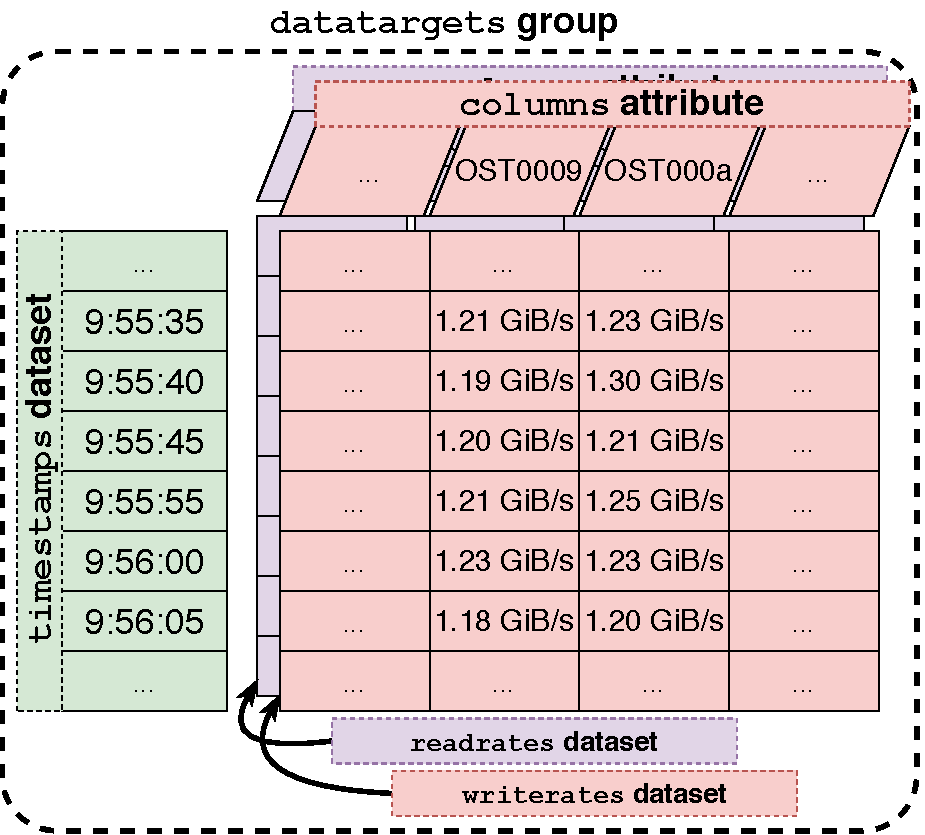
\includegraphics[width=0.9\columnwidth]{tokiotimeseries}
    %\vspace{-.3in}
    \caption{Organization of the \texttt{datatargets} group, which encode traffic to and from file system data targets (Lustre OSTs, GPFS LUNs, or DataWarp NVMe drives), in a TOKIO Time Series file.
    This example reflects read-rate and write-rate data collected from LMT at its native 5-second sampling frequency between 9:55:35 AM and 9:56:05 AM across two OSTs (0x0009 and 0x000a).
    }
    \label{fig:tokiotimeseries}
    \vspace{-.2in}
\end{figure}

\subsubsection{Archival service for real-time data sources}

As described earlier, LMT is a standard component of the Cray ClusterStor software stack which retains high-resolution file system traffic in a MySQL database.
In its most common configuration, LMT retains file system traffic measurements (e.g., bytes read and written) on a per-OST basis every five seconds, but purges this full-resolution data from the MySQL database every 24 hours to prevent the database from becoming untenably large and slow.
To retain these data at full resolution indefinitely, pytokio includes the \texttt{archive\_lmtdb} tool which serializes time series data from the LMT database into an indexed, portable file format called the TOKIO Time Series format.

Based on HDF5, the TOKIO Time Series format organizes time series data from different monitoring tools in their own HDF5 groups, and one such group is schematically depicted in Figure \ref{fig:tokiotimeseries}.
This group (named \texttt{datatargets}) contains two two-dimensional datasets (\texttt{readrates} and \texttt{writerates}) which contain measurements sampled at a fixed frequency.
Each row of these datasets corresponds to a single point in time in the time series (e.g., 9:55:35 AM), and each column corresponds to a single component being measured (e.g., OST \#0009).
To index these datasets in time, a single one-dimensional \texttt{timestamps} dataset is also included in each HDF5 group to describe the absolute times corresponding to each row in the other datasets.
Because data encoded in the TOKIO Time Series format is stored at a fixed frequency for each group, indexing data in time can be done arithmetically using the first timestamp (to establish an absolute reference) and the sampling frequency (to calculate a relative offset).
The columns of each dataset are labeled using an HDF5 dataset attribute which can also be indexed.

The \texttt{archive\_lmtdb} tool that generates these TOKIO Time Series files acts as a bridge between the LMT database connector and the HDF5 connector.
At a high level, it performs data conversion when given a time range and a target LMT database; this core function is supplemented by a thin in-memory caching layer for performance and the logic necessary to ensure the idempotency of updates to existing TOKIO Time Series files.

To automate the archival of LMT data into this TOKIO Time Series format, pytokio's ClusterStor companion repository contains a simple archival service that creates and maintains a library of TOKIO Time Series files that are organized into a date-indexed directory structure.
It creates one TOKIO Time Series file per calendar day, and at a configurable frequency, checks to determine if the day's TOKIO Time Series file is more than an hour out of sync with the LMT database.
If it is, the pytokio archival service uses \texttt{archive\_lmtdb} to retrieve an hour's worth of new data, update the corresponding day's TOKIO Time Series file, and if necessary, roll over to a new day's file.
This service is resilient to falling out of sync with the LMT database due to interruptions in service and has minimal dependencies, allowing it to be easily deployed on any Cray ClusterStor platform.
To date, pytokio and the LMT archival service has been running in production on the Edison XC-30 and Cori XC-40 systems at NERSC and the Theta XC-40 system at the Argonne Leadership Computing Facility. At NERSC, this archival service is deployed full-time using cron jobs, while at the ALCF it is deployed as part of a broader Jenkins-based continuous integration framework.

The pytokio archival service is sufficiently simple and modular to be able to poll and archive the data from any real-time monitoring tool.
For example, NERSC also runs a collectd archival service to retain file system traffic data from the DataWarp burst buffer servers on Cori. 
These burst buffer data are retrieved from NERSC's Elasticsearch-based Data Collect~\cite{Whitney2016} and encoded in TOKIO Time Series files that are schematically identical to those generated by \texttt{archive\_lmtdb}.
Similarly, Lustre failover and fullness data is archived every five minutes using the Lustre LfsOstMap and LfsOstFullness connectors described in Table \ref{tab:connectors}.
In all of these cases, the date-based indexing performed by the pytokio archival service is used to enable the rapid lookup of data from these sources for a given point in time, and in all cases, the archival service runs from an unprivileged account.

\subsubsection{Data services for archived data}

The pytokio archival service provides a mechanism by which high time resolution data can be stored on a file system yet still be quickly accessed via date-based file indexing.
To make these data more accessible to users, pytokio also provides an HDF5 tools interface which serves a very similar function as the Darshan tools interface described in Section \ref{sec:architecture/tools}.
Given a range of time and a file system name, the \texttt{tools.hdf5} interface locates the correct TOKIO Time Series file(s) containing the date ranges requested, loads the relevant datasets, and stitches the data together into pandas DataFrames indexed by time.

While this functionality is exposed via the Python-based \texttt{tools.hdf5} interface, it is very simple to expose these capabilities through a REST API as well.
To demonstrate this, pytokio includes a companion repository that demonstrates a Flask-based application wrapper which exposes the aforementioned \texttt{tools.hdf5} interface as a REST endpoint.
Despite its simplicity, this is an extremely powerful way to connect users with I/O performance data;
for example, JavaScript-based web dashboards can query such a pytokio REST service for JSON-encoded data, then display it as an interactive performance plot using Highcharts or D3.
Similarly, the UMAMI diagram previously described (Figure \ref{fig:umami}) could be statically generated and served on-demand to a web-based frontend to enable quick diagnoses of poorly performing applications.